%
%=====================================================
%
%     Carl Tape, 04-Aug-2007
%     notes.tex
%     last printed xxx
%
%     Notes on converting discrete GPS velocity fields to
%     continuous fields, and then strain rates.
% 
%=====================================================%

\documentclass[11pt,titlepage,fleqn]{article}

\usepackage{amsmath}
\usepackage{amssymb}
\usepackage{latexsym}
\usepackage[round]{natbib}
\usepackage{xspace}
\usepackage{graphicx}
%\usepackage{epsfig}

\usepackage{pifont}   % search for \ding

%\usepackage{fancyhdr}
%\pagestyle{fancy}

%=====================================================
%       SPACING COMMANDS (Latex Companion, p. 52)
%=====================================================

\usepackage{setspace}

\renewcommand{\baselinestretch}{1.3}

\textwidth 460pt
\textheight 690pt
\oddsidemargin 0pt
\evensidemargin 0pt

% see Latex Companion, p. 85
\voffset     -50pt
\topmargin     0pt
\headsep      20pt
\headheight   15pt
\headheight    0pt
\footskip     30pt
\hoffset       0pt

\graphicspath{
  {./figures/}
}

\include{NEWCOMMANDS}

%\newcommand{\figlocA}[1]{/home//carltape/gmt/socal_2005//#1}

%=====================================================
\begin{document}
%=====================================================

\begin{spacing}{1.5}
\begin{center}
{\large \bf Notes on using {\tt surfacevel2strain.m}:

A Matlab program to convert surface velocity fields into strain-rate maps}
\end{center}
\end{spacing}

\bigskip
\noindent Carl Tape, Pablo Mus\'e, Mark Simons

\noindent \today

\small

\begin{verbatim}
surfacevel2strain/USER_INFO/surfacevel2strain_manual.pdf -- this document
surfacevel2strain/USER_INFO/Tape2009gps.pdf              -- GJI2009 
surfacevel2strain/USER_INFO/Tape2009gps_supplement.pdf   -- supplemental notes
surfacevel2strain/matlab/                                -- matlab scripts
\end{verbatim}

%\bigskip
\noindent
Please email Carl Tape ({\tt carltape@gi.alaska.edu}) with suggestions or corrections for the code or these notes.

\tableofcontents

%=====================================================

\section{Introduction}

The purpose of this program is to take an input set of discrete velocity vectors on the surface of a sphere, and then {\em estimate} a continuous velocity vector field on the surface. The estimated field is based on weighted and damped least squares, where the weights are determined from the errors associated with the measurements, but it does not yet use off-axis covariance values.  The program considers 2- or 3-component velocity fields. Several real and synthetic examples were demonstrated in \citet{Tape2009gps}. We suggest testing and understanding \verb+sphereinterp.m+ (\refSec{sec:sphereinterp}), a simpler version for 1D data, prior to using \verb+surfacevel2strain.m+ (\refSec{sec:surfacevel2strain}).

%=====================================================

\section{Example with 1D data: {\tt sphereinterp.m}}
\label{sec:sphereinterp}

In order to demonstrate the basic features of \verb+surfacevel2strain.m+, we will demonstrate the problem of estimating a continuous field on the sphere from a set of discrete 1D observations. The example data are Moho depths derived from receiver functions in southern California \citep{YanClayton2007}, embedded within Moho depths from Crust2.0 \citep{Crust2}. The data sets from these studies are available on-line.

The default example for \verb+sphereinterp.m+ should produce \refFigab{fig:1D_1}{fig:1D_8}, in addition to the text in \refApp{sec:sphereinterp_out}. We will review some of the key steps of the estimation below.
%
\begin{enumerate}
\item Obtain a set of observations and associated uncertainties (\refFig{fig:1D_1}).
\item Obtain the center-points for all basis functions (spherical wavelets) to be used in estimating the continuous field (\refFig{fig:1D_3}). A basis function is kept if a specified number of observation locations is within its spatial support.
\item Obtain a regularization parameter for the inverse problem (\refFig{fig:1D_4}).
\item Solve  least-squares inverse problem for the model vector, which contains coefficients of basis functions. Then compute the estimated field, then analyze the residuals (\refFigii{fig:1D_5}{fig:1D_6}).
\item Using the same model vector, plot the estimated field on a uniform mesh (\refFig{fig:1D_8}). A fancier rendition of \refFig{fig:1D_8} is shown in \refFig{fig:socal_moho}.
\end{enumerate}

%=====================================================

\section{Example with 2D or 3D data: {\tt surfacevel2strain.m}}
\label{sec:surfacevel2strain}

The general procedure is this:
%
\begin{enumerate}
\item Specify a latitude-longitude box for your region of interest. For example, for Japan, we might use:
%
\verb+lonmin0 = 128.0 ; lonmax0 = 147.0 ; latmin0 = 30.0 ; latmax0 = 46.0+
%
This box is used to get the possible wavelet center-points for the estimation, and also to describe the bounds for plotting.

\item Obtain a set of 2- or 3-component velocity field data: $\bv(r_i,\,\theta_i,\,\phi_i)$, where $i$ denotes the index of the observation. Observations outside the bounding region above will be excluded.

\item Save velocity field observations in a ``standard'' format.

\item Specify parameters in \verb+surfacevel2strain.m+ and compute the estimated continuous velocity field.

\item Plot output files in GMT.
\end{enumerate}

%-----------------------

\subsection{Preparing the velocity field dataset ({\tt get\_gps\_dataset.m})}

The most general velocity field dataset is one that contains the data covariances and standard errors.  For a three-component field, the data covariance matrix will have six values per observation.  Thus, for each new dataset, I save a version in a ``standard'' format.
In \verb+get_gps_dataset.m+, the command
%
\begin{verbatim}
[dlon,dlat,ve,vn,vu,se,sn,su,ren,reu,rnu,start_date,finish_date,name] = read_gps_3D(filename);
\end{verbatim}
%
will load the pre-saved GPS dataset.  For the Japan example, see {\tt read\_gps\_japan.m} and {\tt japan\_gps\_dat.m} as a guide.

The variables \verb+start_date+, \verb+finish_date+, and \verb+name+ are not used in \verb+surfacevel2strain.m+. For now, the program does not use the covariance terms \verb+ren+, \verb+reu+, \verb+rnu+.

%-----------------------

\subsection{Running {\tt surfacevel2strain.m}}

We now have simply a set of files, one for each grid $q$, that contain the center-points of what will be spherical wavelet basis functions.

I tested a run using the japan velocity field, considering the horizontal components only (ndim = 2), and performing the estimation for scales \q{0} to \q{8}.

Here is the output to the Matlab command window:
%
%\small
\begin{spacing}{1.0}
\begin{verbatim}
OUTPUT HERE
>>
\end{verbatim}
\end{spacing}
%\normalsize
%
The program prompts the user for various input parameters, and more are needed prior to running the program.  The first run will threshold the basis functions and compute the design matrix for the inverse problem.  There are several ways to select the damping parameter. \refFig{fig:gcv} shows the output figure from \verb+ridge_carl.m+ showing three different parameter selection techniques.

At this point, the inverse problem is done.  Now, the rest of the program is for plotting.  Because computing the design matrix and the damping parameter can be computationally intensive, we do not clear these variables on subsequent runs when we are re-plotting different things.  In other words, we now execute the program again:
%
%\small
\begin{spacing}{1.0}
\begin{verbatim}
>>
\end{verbatim}
\end{spacing}
%\normalsize
%
The output is a set of figures showing the estimated velocity fields, as well as scalar fields derived from the spatial velocity gradient tensor field, $\bL(\phi, \theta)$.

%-----------------------

%\pagebreak
\subsection*{Plotting scalar and vector fields in GMT}

There are several \verb+perl+ scripts for plotting in GMT here:
%
\verb+surfacevel2strain/gmt/util/+.
%
These will require several modifications for your own purposes. The primary script to run is \verb+plot_strain.pl+.

Example output figures are shown in \refFigab{fig:japan_vel_no_mask}{fig:japan_strain}.

%=====================================================
%\pagebreak
%\small
\addcontentsline{toc}{section}{References}
\bibliographystyle{agu08}
\bibliography{preamble,REFERENCES,refs_socal,refs_carl}

%=====================================================

\appendix
\section{Output from {\tt sphereinterp.m}}
\label{sec:sphereinterp_out}

Below is the output generated to the Matlab command window in the process of generating \refFigab{fig:1D_1}{fig:1D_8} (\refSec{sec:sphereinterp}).

%\small
\begin{spacing}{1.0}
\begin{verbatim}
 Type an index corresponding to a region (1=socal): 1
 Type an index corresponding to a dataset (1=moho): 1
getsubset.m: 124 points in the subset out of 124
------------------------------------------------------------
entering sphereinterp_grid.m to obtain spherical wavelet basis functions
Support of the spherical wavelets:
   q      deg           km
   0     82.442     9167.1
   1     47.310     5260.7
   2     24.707     2747.3
   3     12.500     1389.9
   4      6.268      697.0
   5      3.136      348.8
   6      1.569      174.4
   7      0.784       87.2
   8      0.392       43.6
   9      0.196       21.8
  10      0.103       11.4
  11      0.052        5.8
  12      0.026        2.9
  
minimum allowable grid order is 3
   1.39e+06 meters (support of q = 3 wavelet) < 1.94e+06 meters (2*Lscale)
getspheregrid.m: lon-lat subregion of sphere
  
GRID ORDER q = 3
  dbase = 7.929e+00 deg
  lonmin, lonmax, latmin, latmax:
  -145.79, -89.21, 6.21, 61.79
  phmin, phmax, thmin, thmax:
  -2.5445, -1.5570, 0.4924, 1.4624
Patch occupies this fraction of the sphere: 6.074e-02
This corresponds to a square patch with side length 50.057 deg
getting the gridpoints for q = 3
  number of total possible gridpoints : 642
  maximum number of subset gridpoints : 39
q = 3, nf = 8, dbase = 7.929e+00 deg
  actual number of subset gridpoints : 42
  
GRID ORDER q = 4
  dbase = 3.965e+00 deg
  lonmin, lonmax, latmin, latmax:
  -133.89, -101.11, 18.11, 49.89
  phmin, phmax, thmin, thmax:
  -2.3369, -1.7646, 0.7000, 1.2548
Patch occupies this fraction of the sphere: 2.068e-02
This corresponds to a square patch with side length 29.207 deg
getting the gridpoints for q = 4
  number of total possible gridpoints : 2562
  maximum number of subset gridpoints : 53
q = 4, nf = 16, dbase = 3.965e+00 deg
  actual number of subset gridpoints : 53
  
GRID ORDER q = 5
  dbase = 1.982e+00 deg
  lonmin, lonmax, latmin, latmax:
  -127.95, -107.05, 24.05, 43.95
  phmin, phmax, thmin, thmax:
  -2.2331, -1.8684, 0.8038, 1.1510
Patch occupies this fraction of the sphere: 8.312e-03
This corresponds to a square patch with side length 18.517 deg
getting the gridpoints for q = 5
  number of total possible gridpoints : 10242
  maximum number of subset gridpoints : 85
q = 5, nf = 32, dbase = 1.982e+00 deg
  actual number of subset gridpoints : 78
  
GRID ORDER q = 6
  dbase = 9.912e-01 deg
  lonmin, lonmax, latmin, latmax:
  -124.97, -110.03, 27.03, 40.97
  phmin, phmax, thmin, thmax:
  -2.1812, -1.9203, 0.8557, 1.0991
Patch occupies this fraction of the sphere: 4.179e-03
This corresponds to a square patch with side length 13.130 deg
getting the gridpoints for q = 6
  number of total possible gridpoints : 40962
  maximum number of subset gridpoints : 171
q = 6, nf = 64, dbase = 9.912e-01 deg
  actual number of subset gridpoints : 158
  
GRID ORDER q = 7
  dbase = 4.956e-01 deg
  lonmin, lonmax, latmin, latmax:
  -123.49, -111.51, 28.51, 39.49
  phmin, phmax, thmin, thmax:
  -2.1553, -1.9463, 0.8816, 1.0731
Patch occupies this fraction of the sphere: 2.636e-03
This corresponds to a square patch with side length 10.429 deg
getting the gridpoints for q = 7
  number of total possible gridpoints : 163842
  maximum number of subset gridpoints : 432
q = 7, nf = 128, dbase = 4.956e-01 deg
  actual number of subset gridpoints : 401
  
GRID ORDER q = 8
  dbase = 2.478e-01 deg
  lonmin, lonmax, latmin, latmax:
  -122.74, -112.26, 29.26, 38.74
  phmin, phmax, thmin, thmax:
  -2.1423, -1.9592, 0.8946, 1.0602
Patch occupies this fraction of the sphere: 1.997e-03
This corresponds to a square patch with side length 9.077 deg
getting the gridpoints for q = 8
  number of total possible gridpoints : 655362
  maximum number of subset gridpoints : 1309
q = 8, nf = 256, dbase = 2.478e-01 deg
  actual number of subset gridpoints : 1216
  
 threshold the gridpoints
  
     q   num    id    i1    i2
     3    12    12     1    12
     4    14    26    13    26
     5    24    50    27    50
     6    45    95    51    95
     7    77   172    96   172
     8   102   274   173   274
  
GRIDPOINTS q = 3 to 8 (274):
274 wavelets / 1948 total with >= 3 stations inside their corresponding spatial supports
  
 q = 3 to 8, j = 1 to 274 (274)
 q = 3 to 6, j = 1 to 95 (95)
 q = 7 to 7, j = 96 to 172 (77)
 q = 8 to 8, j = 173 to 274 (102)
------------------------------------------------------------
entering sphereinterp_est.m to estimate smooth scalar field on the sphere
no input polygon provided --> full plotting grid will be used
choice of regularization parameter:
ordinary cross validation
input uncertainties will be used within inversion
  
Constructing the design matrix...
 creating the L-curve...
 ii = 1/40, lam = 0.001
 ii = 2/40, lam = 0.0017013
   :
 ii = 37/40, lam = 203091.7621
 ii = 38/40, lam = 345510.7295
 ii = 39/40, lam = 587801.6072
 ii = 40/40, lam = 1000000
  
Pick the regularization parameter:
L-curve lambda = 7.017e-02 (index 9)
    OCV lambda = 3.455e-01 (index 12)
    GCV lambda = 2.031e-01 (index 11)
your pick lam0 = 3.455e-01 (index 12)
 computing the model vector...
  
 computing values at the plotting points...
100 out of 2200
  :
2200 out of 2200
Elapsed time is 15.812080 seconds.
  
Number of observations, ndata = 124
Number of basis functions, ngrid = 274
For testing purposes, try decreasing one of these:
  qmax = 8, the densest grid for basis functions
  nx = 50, the grid density for plotting
  ndata = 124, the number of observations (or ax0)
>> 
\end{verbatim}
\end{spacing}
%\normalsize

%-------------------------------------------------------

\section{Output from {\tt surfacevel2strain.m}}
\label{sec:sphereinterp_out}

Below is the output generated to the Matlab command window in the process of generating \refFigab{fig:2D_A5}{fig:2D_A7}, among many more (\refSec{sec:surfacevel2strain}).

%\small
\begin{spacing}{1.0}
\begin{verbatim}
 Type 1 for new inversion or 0 otherwise: 1
 Type 1 to use spherical wavelets, 2 for spherical splines: 1
 Type 1 to use the DIAGONAL covariance matrix for weighting (0 otherwise): 1
 Type the number of components of the v-field for the inversion (2 or 3) : 2
 Type 1 to plot with the mask (0 otherwise) : 1
 Type 1 to write output to files for GMT plotting (0 otherwise) : 0
 Type an index corresponding to a region (1=us, 2=cal, 3=socal, ..., 8=parkfield): 3
 Type an index corresponding to a v-field dataset (1=REASON): 1
read_gps_3D.m: /home/carltape/compearth/surfacevel2strain/data/examples/reason_subset_3D.dat
getsubset.m: 408 points in the subset out of 510
tp2xyz.m: uniform radial value
 Type 1 to remove a uniform rotation, 0 otherwise: 1
tp2xyz.m: uniform radial value
Support of the spherical wavelets:
   q      deg           km
   0     82.442     9167.1
   1     47.310     5260.7
   2     24.707     2747.3
   3     12.500     1389.9
   4      6.268      697.0
   5      3.136      348.8
   6      1.569      174.4
   7      0.784       87.2
   8      0.392       43.6
   9      0.196       21.8
  10      0.103       11.4
  11      0.052        5.8
  12      0.026        2.9
  
minimum allowable grid order is 3
   1.39e+06 meters (support of q = 3 wavelet) < 1.94e+06 meters (2*Lscale)
 Type min allowable grid order, qmin >= 0 (try 3): 3
 Type max allowable grid order, qmax: 7
getspheregrid.m: lon-lat subregion of sphere
  
GRID ORDER q = 3
  dbase = 7.929e+00 deg
  lonmin, lonmax, latmin, latmax:
  -145.79, -89.21, 6.21, 61.79
  phmin, phmax, thmin, thmax:
  -2.5445, -1.5570, 0.4924, 1.4624
Patch occupies this fraction of the sphere: 6.074e-02
This corresponds to a square patch with side length 50.057 deg
getting the gridpoints for q = 3
  number of total possible gridpoints : 642
  maximum number of subset gridpoints : 39
q = 3, nf = 8, dbase = 7.929e+00 deg
  actual number of subset gridpoints : 42
  
GRID ORDER q = 4
  dbase = 3.965e+00 deg
  lonmin, lonmax, latmin, latmax:
  -133.89, -101.11, 18.11, 49.89
  phmin, phmax, thmin, thmax:
  -2.3369, -1.7646, 0.7000, 1.2548
Patch occupies this fraction of the sphere: 2.068e-02
This corresponds to a square patch with side length 29.207 deg
getting the gridpoints for q = 4
  number of total possible gridpoints : 2562
  maximum number of subset gridpoints : 53
q = 4, nf = 16, dbase = 3.965e+00 deg
  actual number of subset gridpoints : 53
  
GRID ORDER q = 5
  dbase = 1.982e+00 deg
  lonmin, lonmax, latmin, latmax:
  -127.95, -107.05, 24.05, 43.95
  phmin, phmax, thmin, thmax:
  -2.2331, -1.8684, 0.8038, 1.1510
Patch occupies this fraction of the sphere: 8.312e-03
This corresponds to a square patch with side length 18.517 deg
getting the gridpoints for q = 5
  number of total possible gridpoints : 10242
  maximum number of subset gridpoints : 85
q = 5, nf = 32, dbase = 1.982e+00 deg
  actual number of subset gridpoints : 78
  
GRID ORDER q = 6
  dbase = 9.912e-01 deg
  lonmin, lonmax, latmin, latmax:
  -124.97, -110.03, 27.03, 40.97
  phmin, phmax, thmin, thmax:
  -2.1812, -1.9203, 0.8557, 1.0991
Patch occupies this fraction of the sphere: 4.179e-03
This corresponds to a square patch with side length 13.130 deg
getting the gridpoints for q = 6
  number of total possible gridpoints : 40962
  maximum number of subset gridpoints : 171
q = 6, nf = 64, dbase = 9.912e-01 deg
  actual number of subset gridpoints : 158
  
GRID ORDER q = 7
  dbase = 4.956e-01 deg
  lonmin, lonmax, latmin, latmax:
  -123.49, -111.51, 28.51, 39.49
  phmin, phmax, thmin, thmax:
  -2.1553, -1.9463, 0.8816, 1.0731
Patch occupies this fraction of the sphere: 2.636e-03
This corresponds to a square patch with side length 10.429 deg
getting the gridpoints for q = 7
  number of total possible gridpoints : 163842
  maximum number of subset gridpoints : 432
q = 7, nf = 128, dbase = 4.956e-01 deg
  actual number of subset gridpoints : 401
  
 threshold the gridpoints
  
     q   num    id    i1    i2
     3    11    11     1    11
     4    15    26    12    26
     5    25    51    27    51
     6    52   103    52   103
     7   124   227   104   227
 Enter max q grid for secular field (3 <= qsec <= 7): 5
  
Thresholding GRIDPOINTS q = 3 to 7 (227):
227 wavelets / 732 total with >= 3 stations inside their corresponding spatial supports
  
 q = 3 to 7, j = 1 to 227 (227)
 q = 3 to 5, j = 1 to 51 (51)
 q = 6 to 6, j = 52 to 103 (52)
 q = 7 to 7, j = 104 to 227 (124)
  
Constructing the design matrix...
regularization curves for scalar field vsouth
 ii = 1/40, lam = 0.001
 ii = 2/40, lam = 0.0017013
  :
 ii = 39/40, lam = 587801.6072
 ii = 40/40, lam = 1000000
L-curve lambda = 4.924e+03 (index 30)
    OCV lambda = 1.701e+03 (index 28)
    GCV lambda = 2.424e-02 (index 7)
Type an index for lambda (try iOCV = 28): 28
regularization curves for scalar field veast
 ii = 1/40, lam = 0.001
 ii = 2/40, lam = 0.0017013
  :
 ii = 39/40, lam = 587801.6072
 ii = 40/40, lam = 1000000
L-curve lambda = 4.924e+03 (index 30)
    OCV lambda = 1.701e+03 (index 28)
    GCV lambda = 7.017e+01 (index 22)
Type an index for lambda (try iOCV = 28): 28
  
 got the regularization parameters (vr, vth, vphi):
    lam0 = NaN 1.70e+03 1.70e+03
>> 
\end{verbatim}
\end{spacing}
%\normalsize

\noindent
At this point, the design matrix has been constructed and the regularization parameter has been selected. To avoid recomputing these quantities, the user is given the option to plot and analyze results while changing additional parameters. Below is the output generated to the Matlab command window in the process of generating \refFigab{fig:2D_B03}{fig:2D_B06}, among many more (\refSec{sec:surfacevel2strain}).

%\small
\begin{spacing}{1.0}
\begin{verbatim}
 Type 1 for new inversion or 0 otherwise: 0
  
 computing the model vector...
surfacevel2strain_figs.m: plotting with ifigs1==1
  
Constructing the base design matrix for plotting...
 computing a mask for plotting...
3918 out of 8800 plotting points are unmasked
 compute L : assume isotropic linear elasticity, Poisson solid, and surface condition
surfacevel2strain_evec.m: computing euler vectors...
 Enter minimum value of omega for euler vectors (default = 0 rad/yr): 1.5e-7
tp2xyz.m: uniform radial value
tp2xyz.m: uniform radial value
 computing the max eigenvalue at each point...
surfacevel2strain_figs.m: plotting with ifigs2==1
 plotting velocities at different scales ...
 plotting strain maps...
    1.0000    0.0246
    2.0000    0.0269
    3.0000    1.6246
    4.0000    1.9438
    5.0000    1.3046
    6.0000    1.8954
 plotting components of the scalar quantity STRAIN...
    1.0000    0.0000
    2.0000    0.0000
    3.0000    0.0000
    5.0000    0.0000
    6.0000    0.0000
1  2.9750e-07
2  3.1625e-07
3  1.2570e-07
4  1.3862e-07
5  2.4027e-07
6  4.2046e-07
1  -1.2570e-07
2  4.2046e-07
3  2.4027e-07
4  3.2916e-07
exiting surfacevel2strain_figs.m
DONE with surfacevel2strain.m
>> 
\end{verbatim}
\end{spacing}
%\normalsize

%=====================================================

\normalsize

\clearpage\pagebreak
\begin{figure}
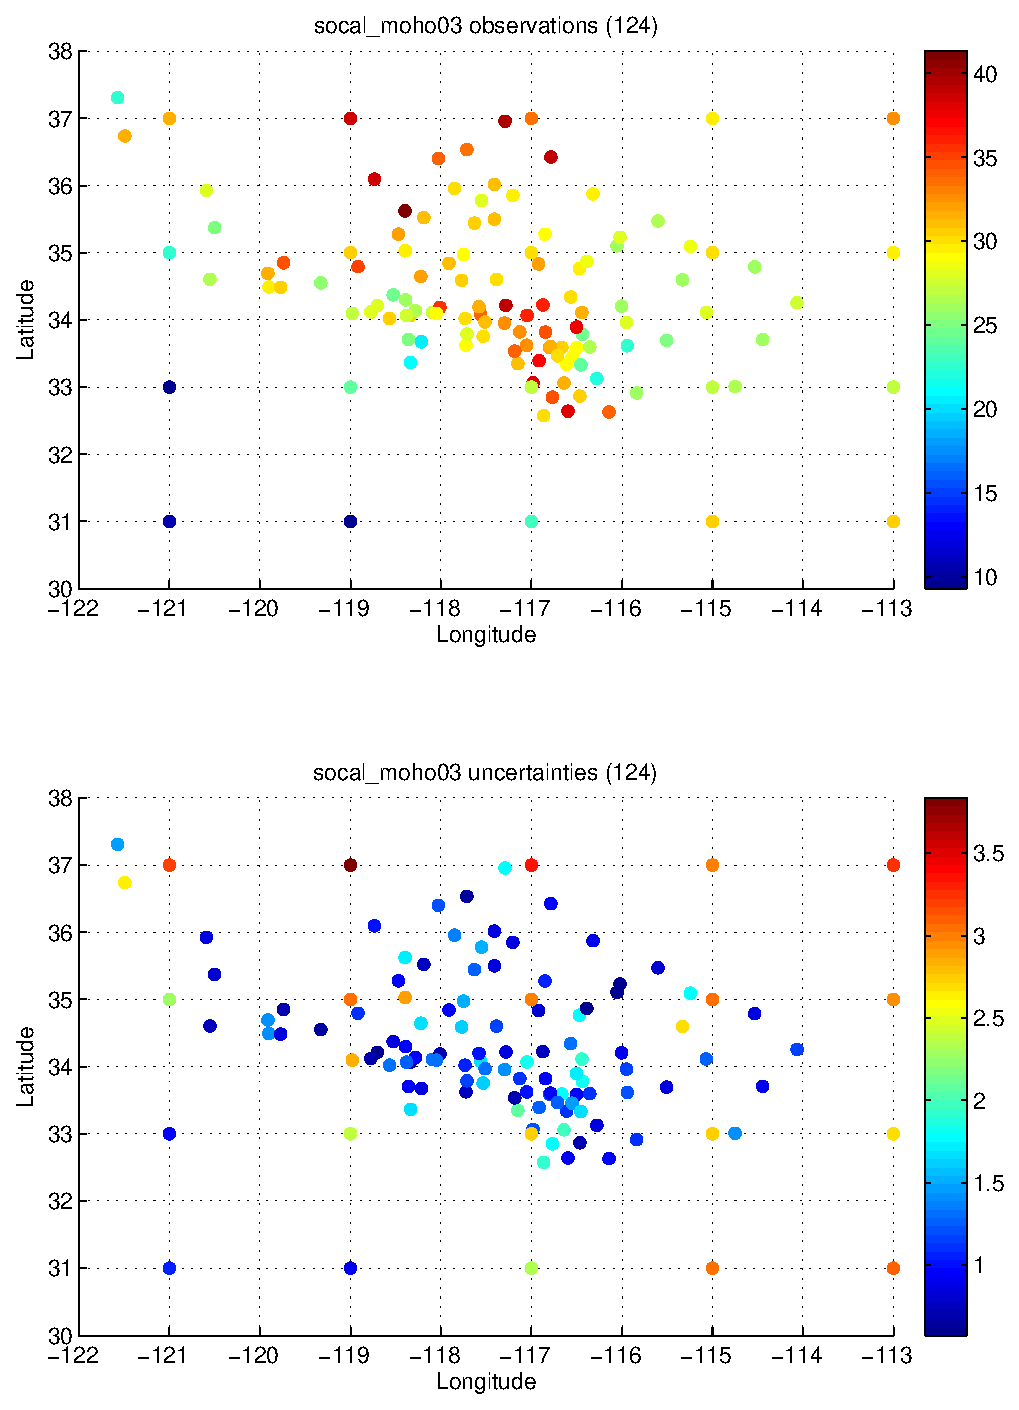
\includegraphics[width=15cm]{fig1D_1.eps}
\caption[]
{{
Example 1D data set for estimating a continuous function on the sphere (\refSec{sec:sphereinterp}).
The data set is comprised of Moho depth estimates at discrete locations.
The top plot is for the Moho depth, and the bottom plot is for the estimated uncertainty associated with each depth. Values are from \citet{YanClayton2007} and \citet{Crust2}.
\label{fig:1D_1}
}}
\end{figure}

\begin{figure}
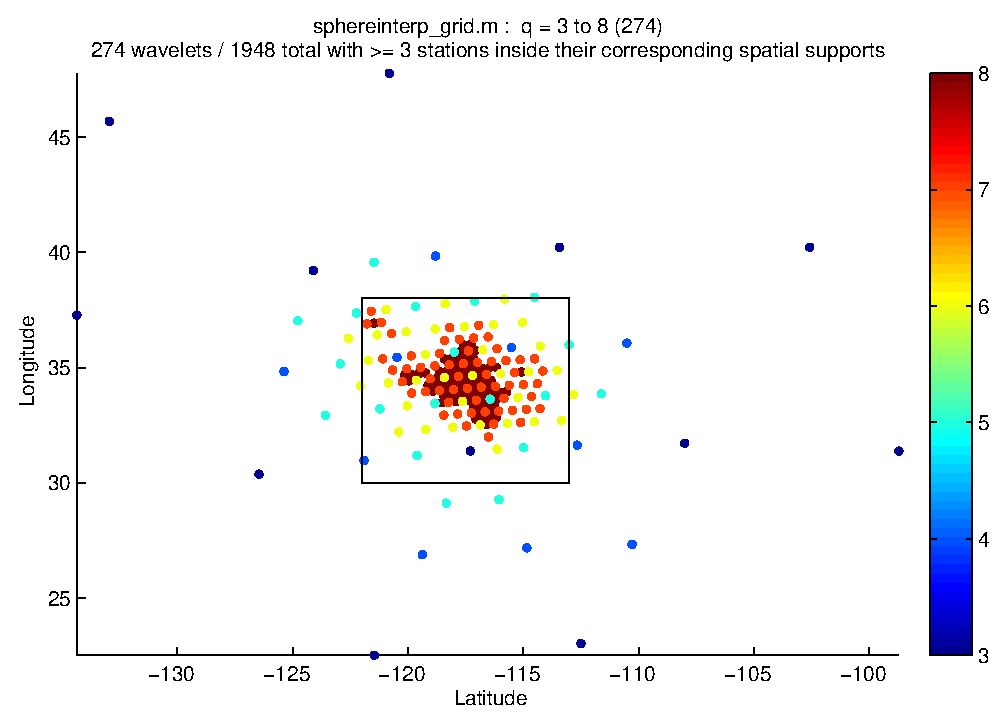
\includegraphics[width=16cm]{fig1D_2.eps}
\caption[]
{{
Full set of center-points for basis functions used in the inversion.
Color corresponds to the scale $q$ for each basis function.
Note that some dots correspond to multiple basis functions with different scales $q$, but only the highest-$q$ is visible.
See partition by scale in \refFig{fig:1D_3}.
\label{fig:1D_2}
}}
\end{figure}

\begin{figure}
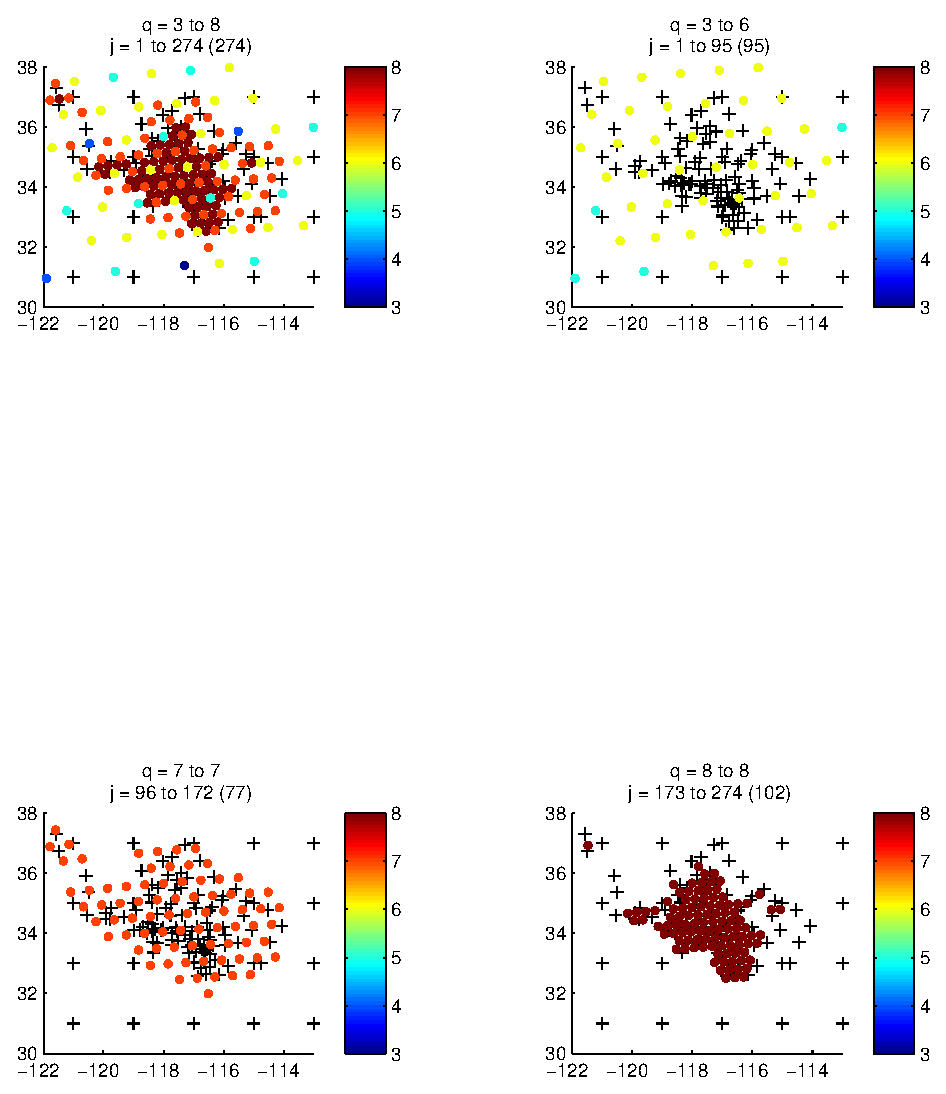
\includegraphics[width=16cm]{fig1D_3.eps}
\caption[]
{{
Basis function gridpoint centers for grids \q{3-8} (\refFig{fig:1D_2}), \q{3-6}, \q{7}, and \q{8}.
Color corresponds to the scale $q$ for each basis function.
Observation locations are plotted at `+' markers (\refFig{fig:1D_1}).
\label{fig:1D_3}
}}
\end{figure}

\begin{figure}
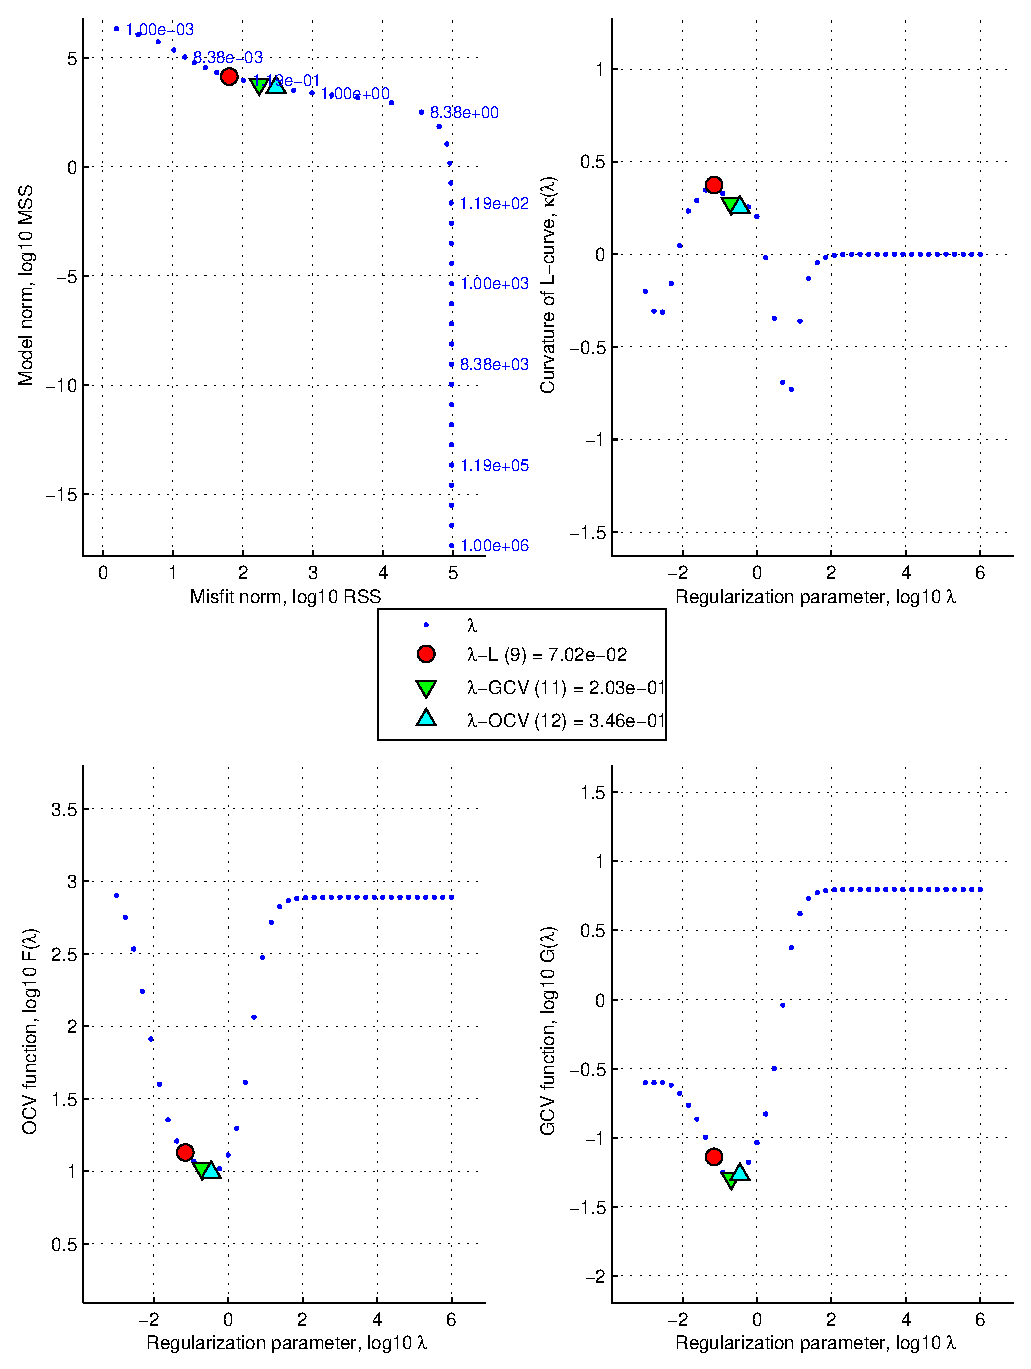
\includegraphics[width=16cm]{fig1D_4.eps}
\caption[]
{{
Selection of regularization parameter, $\lambda$, considering three different approaches: L-curve, ordinary cross-validation, general cross-validation. See \citet{Tape2009gps} for details and references. For this example, all three techniques select a similar regularization paramter.
\label{fig:1D_4}
}}
\end{figure}

\begin{figure}
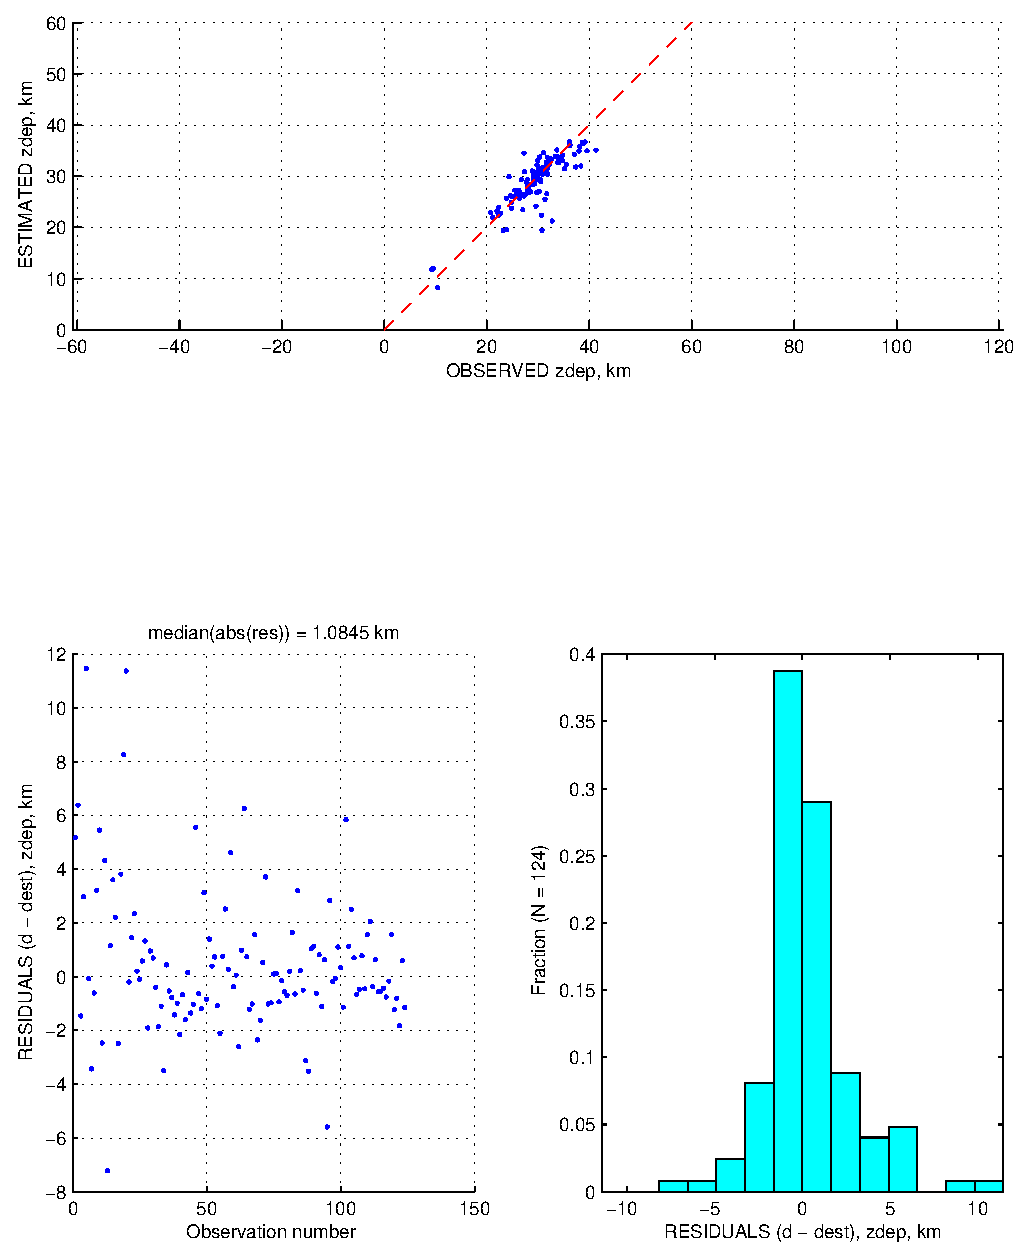
\includegraphics[width=16cm]{fig1D_5.eps}
\caption[]
{{
Comparison between observations and predictions for the 124 Moho depths.
\label{fig:1D_5}
}}
\end{figure}

\begin{figure}
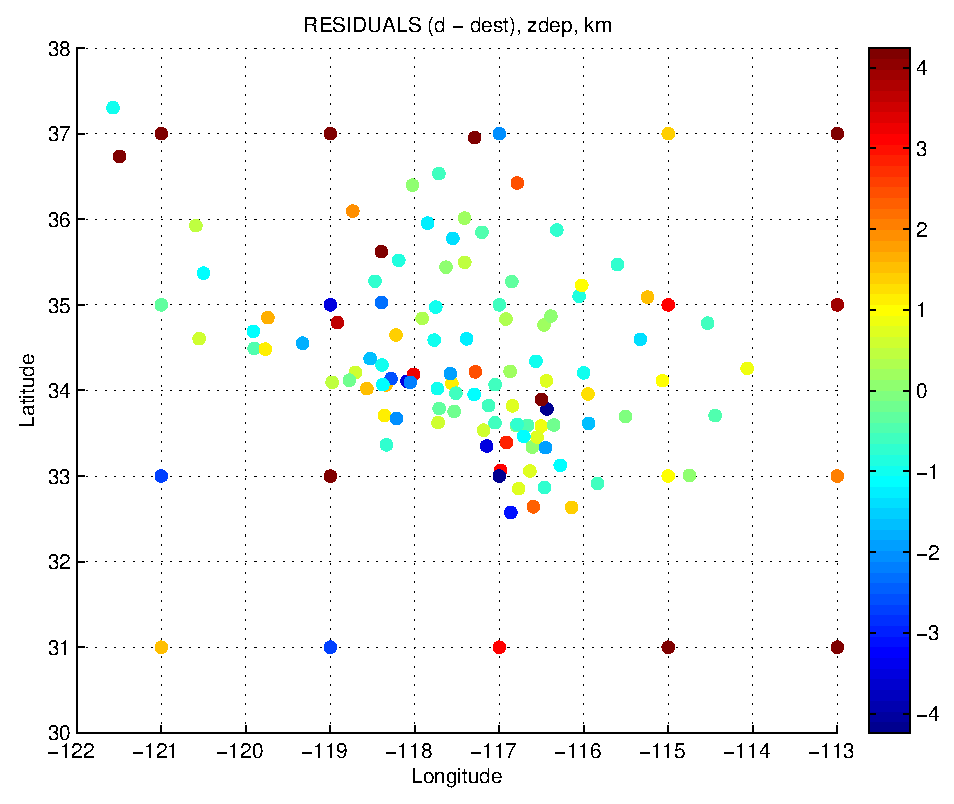
\includegraphics[width=16cm]{fig1D_6.eps}
\caption[]
{{
Spatial plot of residuals between observed and estimated Moho depths.
\label{fig:1D_6}
}}
\end{figure}

\begin{figure}
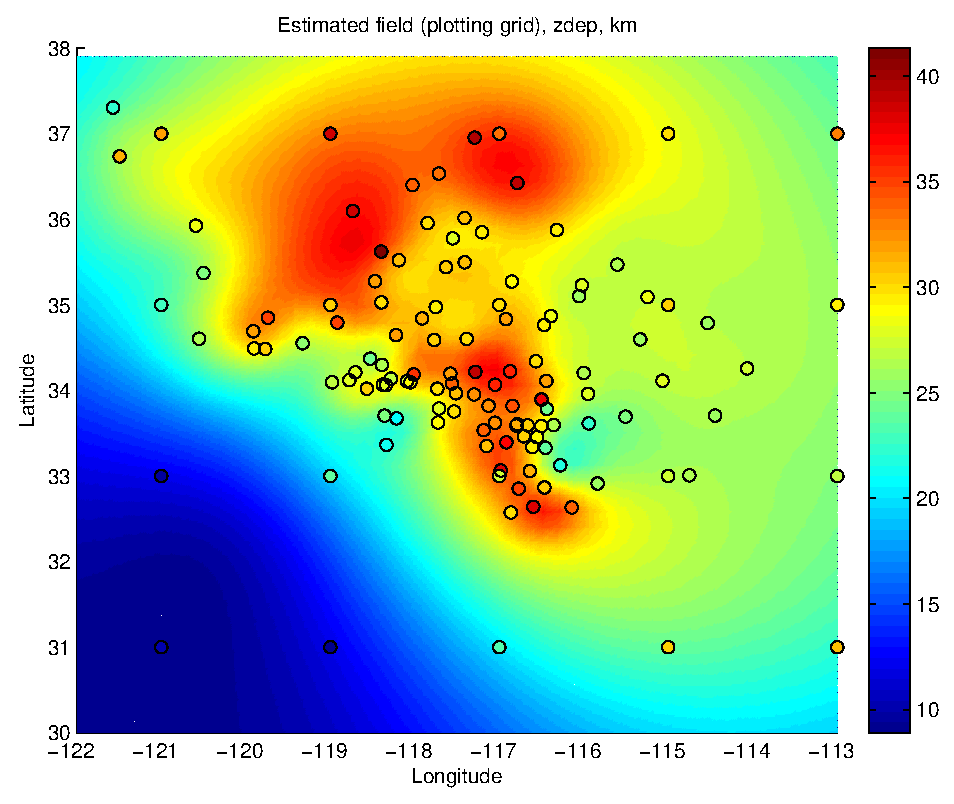
\includegraphics[width=16cm]{fig1D_8.eps}
\caption[]
{{
Estimated field, with observed values plotted as circles.
\label{fig:1D_8}
}}
\end{figure}

\begin{figure}
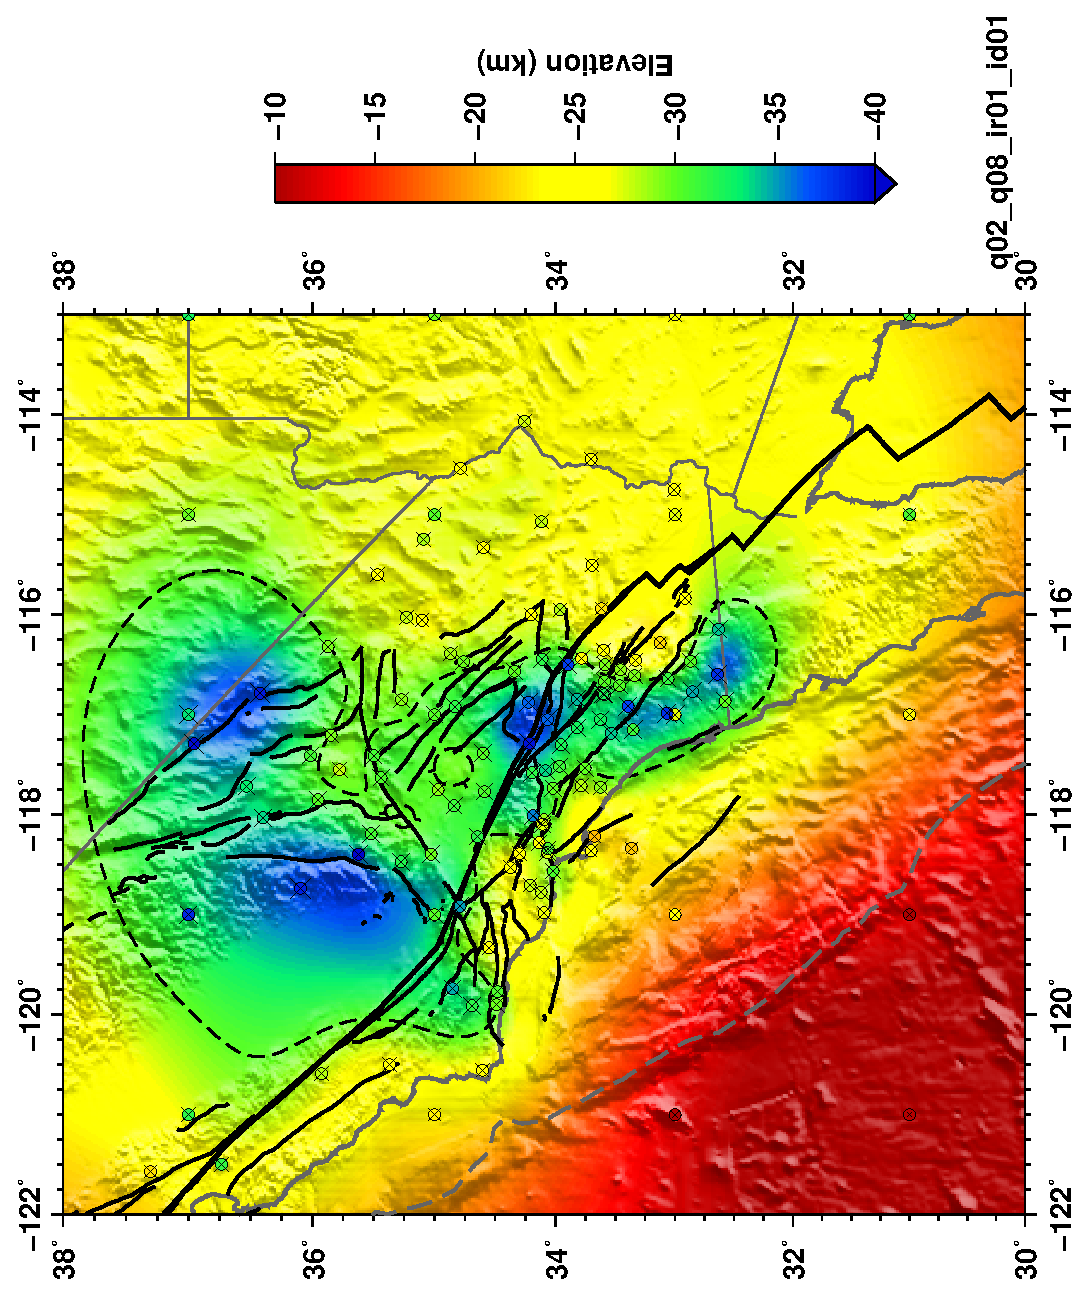
\includegraphics[width=14cm,angle=-90]{socal_moho03_q02_q08.eps}
\caption[]
{{
A fancier rendition of \refFig{fig:1D_8}. The dashed line shows the $-30$~km contour.
Each filled circle is an observed values, with the `x' marker proportional to the uncertainty.
\label{fig:socal_moho}
}}
\end{figure}

%-----------------------------------------------------

\begin{figure}
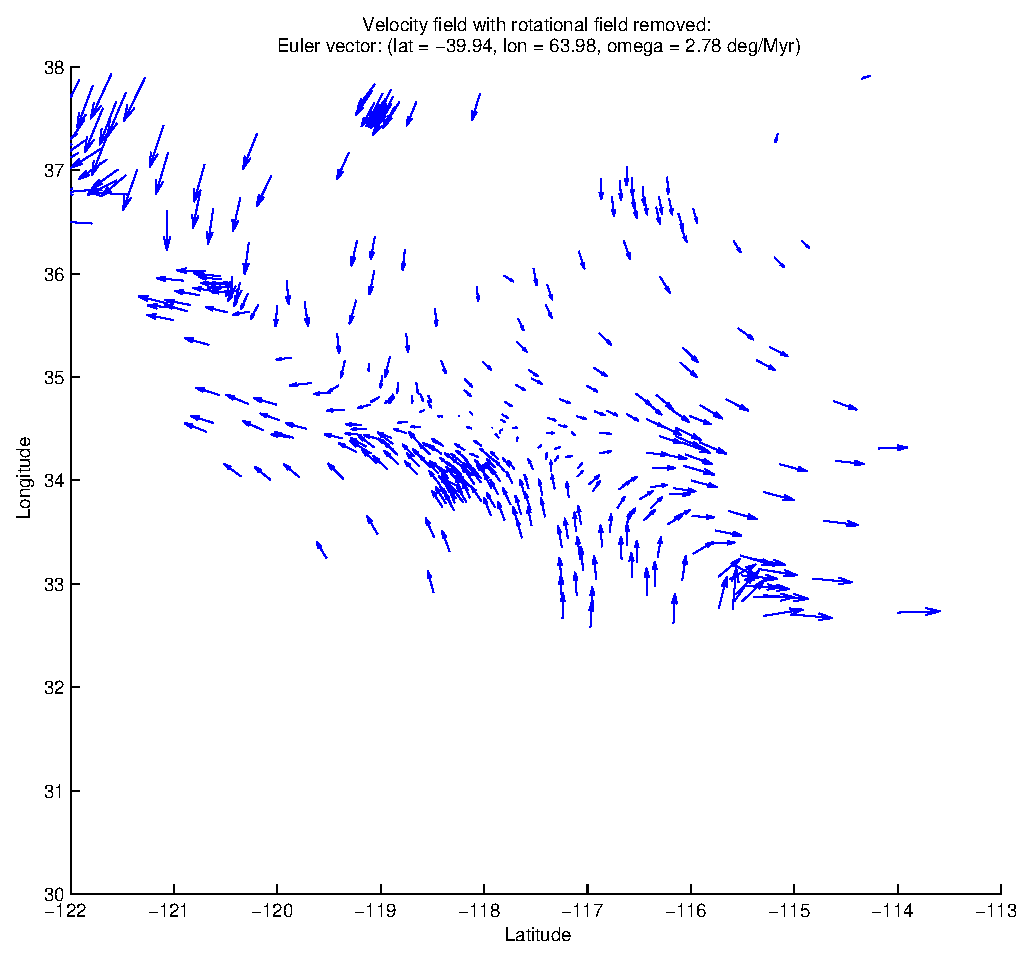
\includegraphics[width=16cm]{fig2D_A5.eps}
\caption[]
{{
Text.
\label{fig:2D_A5}
}}
\end{figure}

\begin{figure}
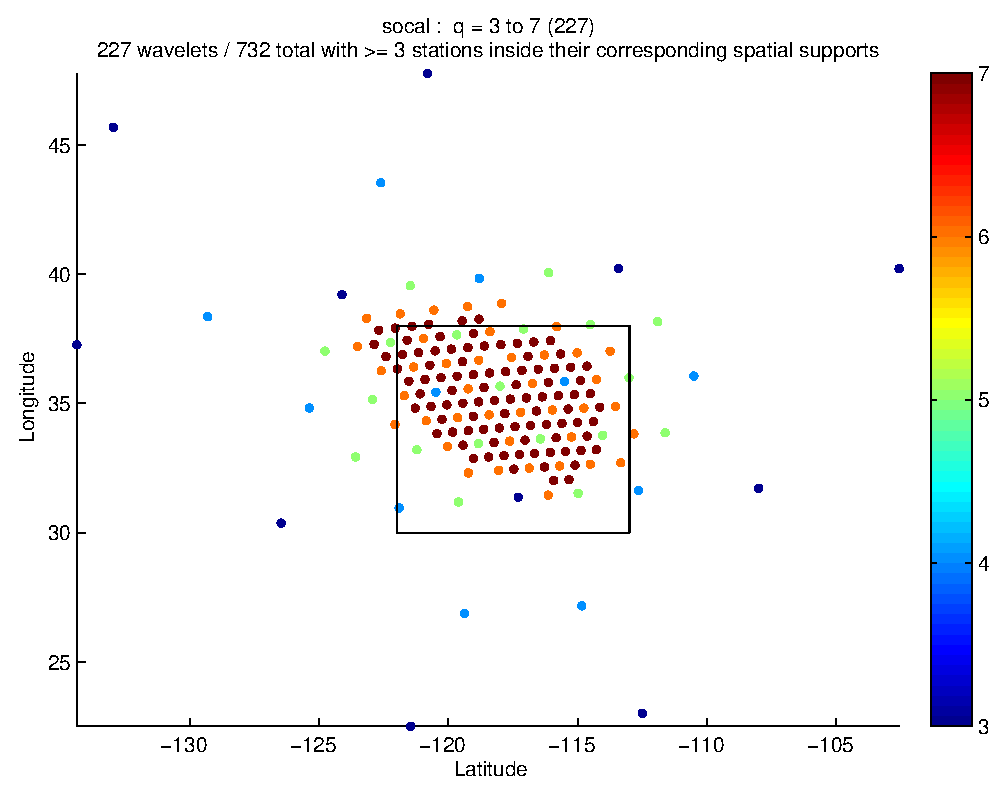
\includegraphics[width=16cm]{fig2D_A6.eps}
\caption[]
{{
Text.
\label{fig:2D_A6}
}}
\end{figure}

\begin{figure}
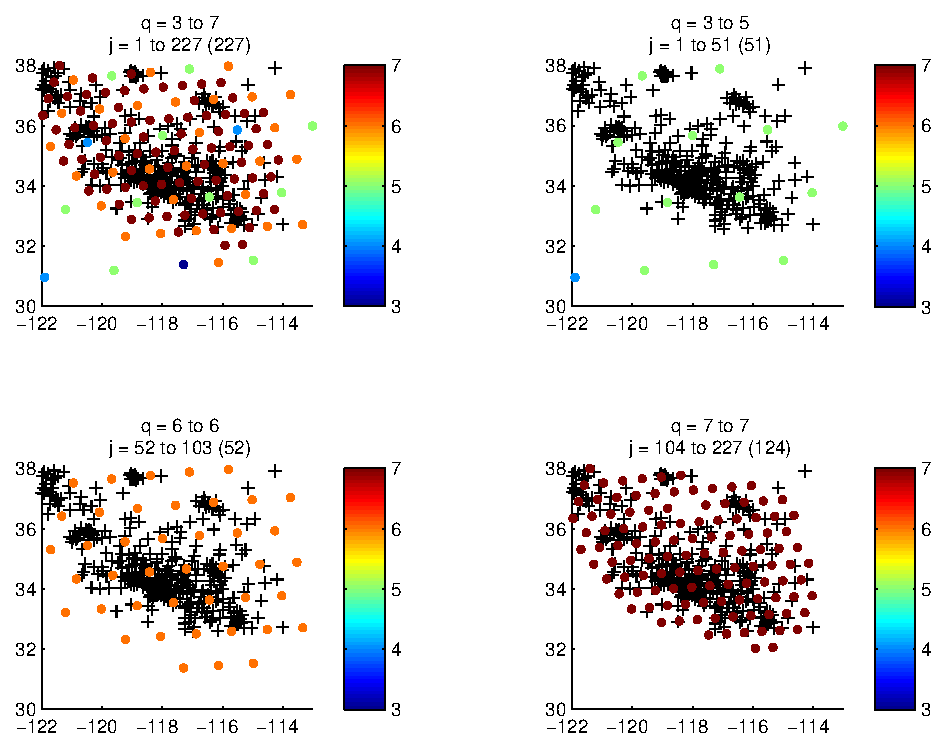
\includegraphics[width=16cm]{fig2D_A7.eps}
\caption[]
{{
Text.
\label{fig:2D_A7}
}}
\end{figure}

\begin{figure}
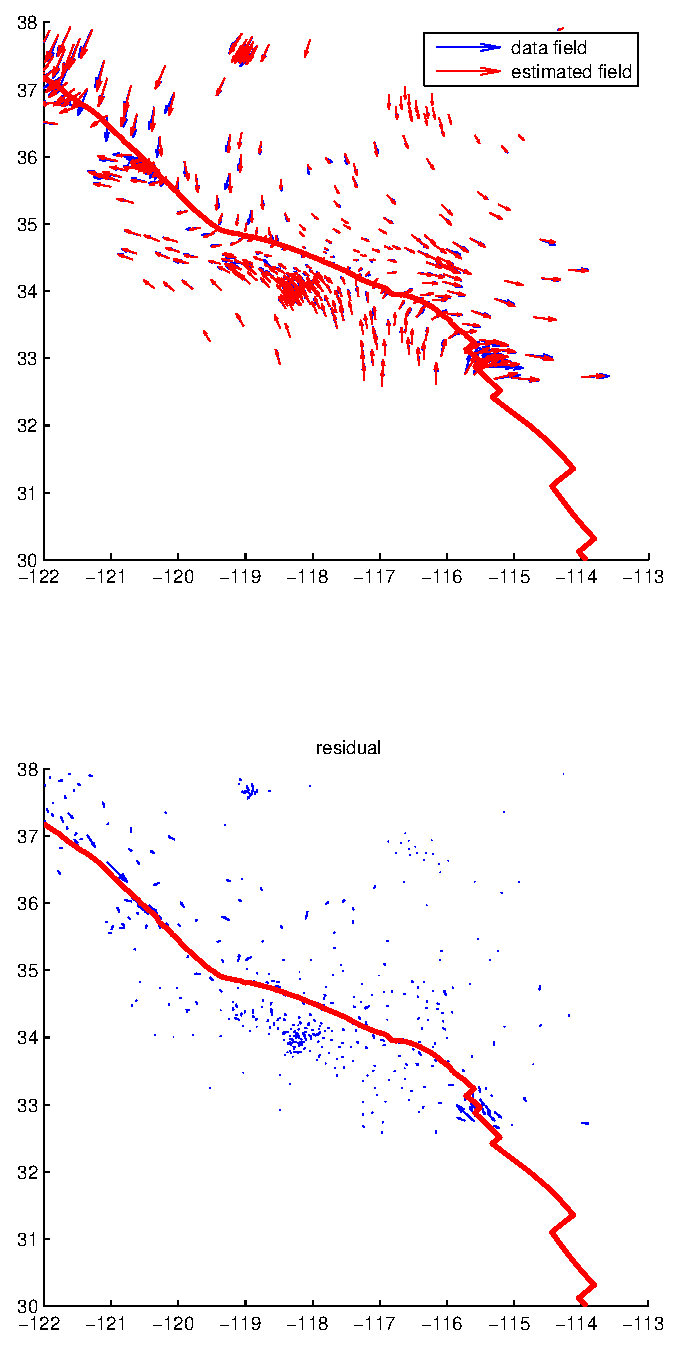
\includegraphics[width=12cm]{fig2D_B03.eps}
\caption[]
{{
Text.
\label{fig:2D_B03}
}}
\end{figure}

\begin{figure}
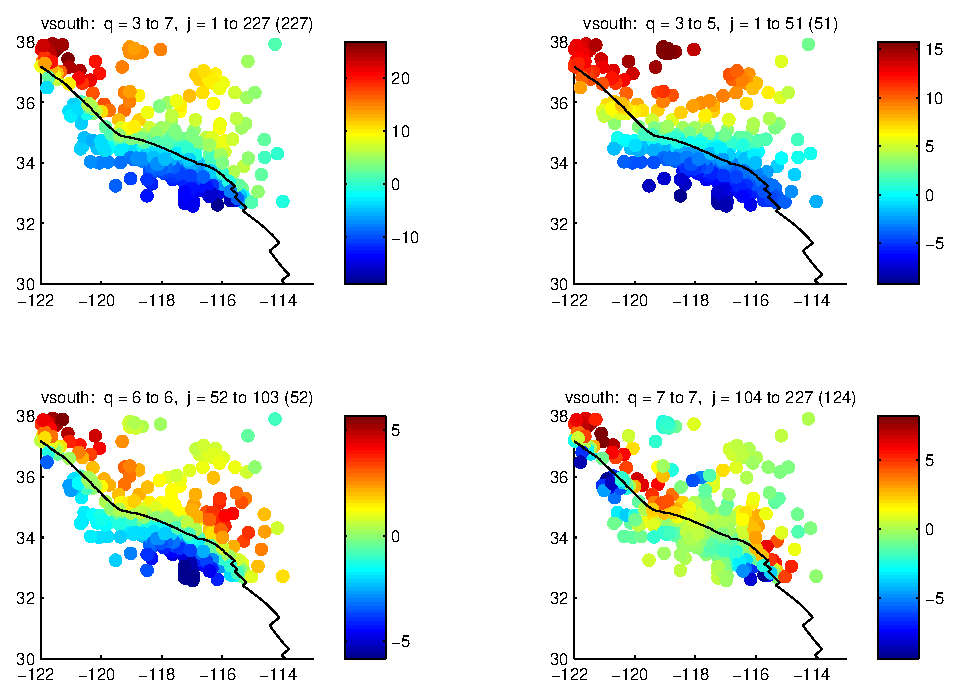
\includegraphics[width=16cm]{fig2D_B05.eps}
\caption[]
{{
Text.
\label{fig:2D_B03}
}}
\end{figure}

\begin{figure}
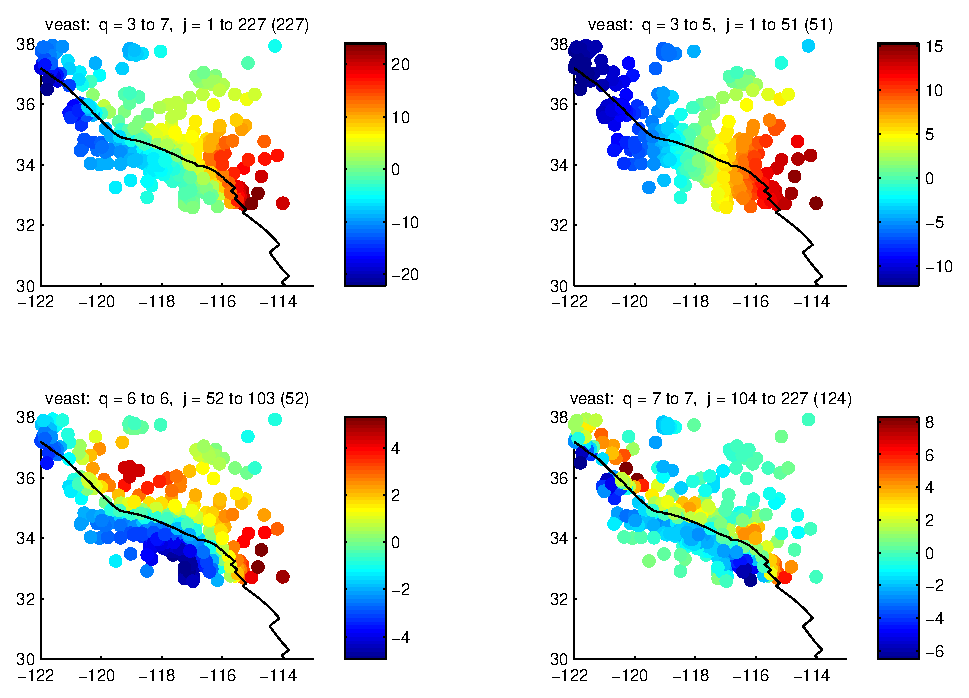
\includegraphics[width=16cm]{fig2D_B06.eps}
\caption[]
{{
Text.
\label{fig:2D_B03}
}}
\end{figure}

\begin{figure}
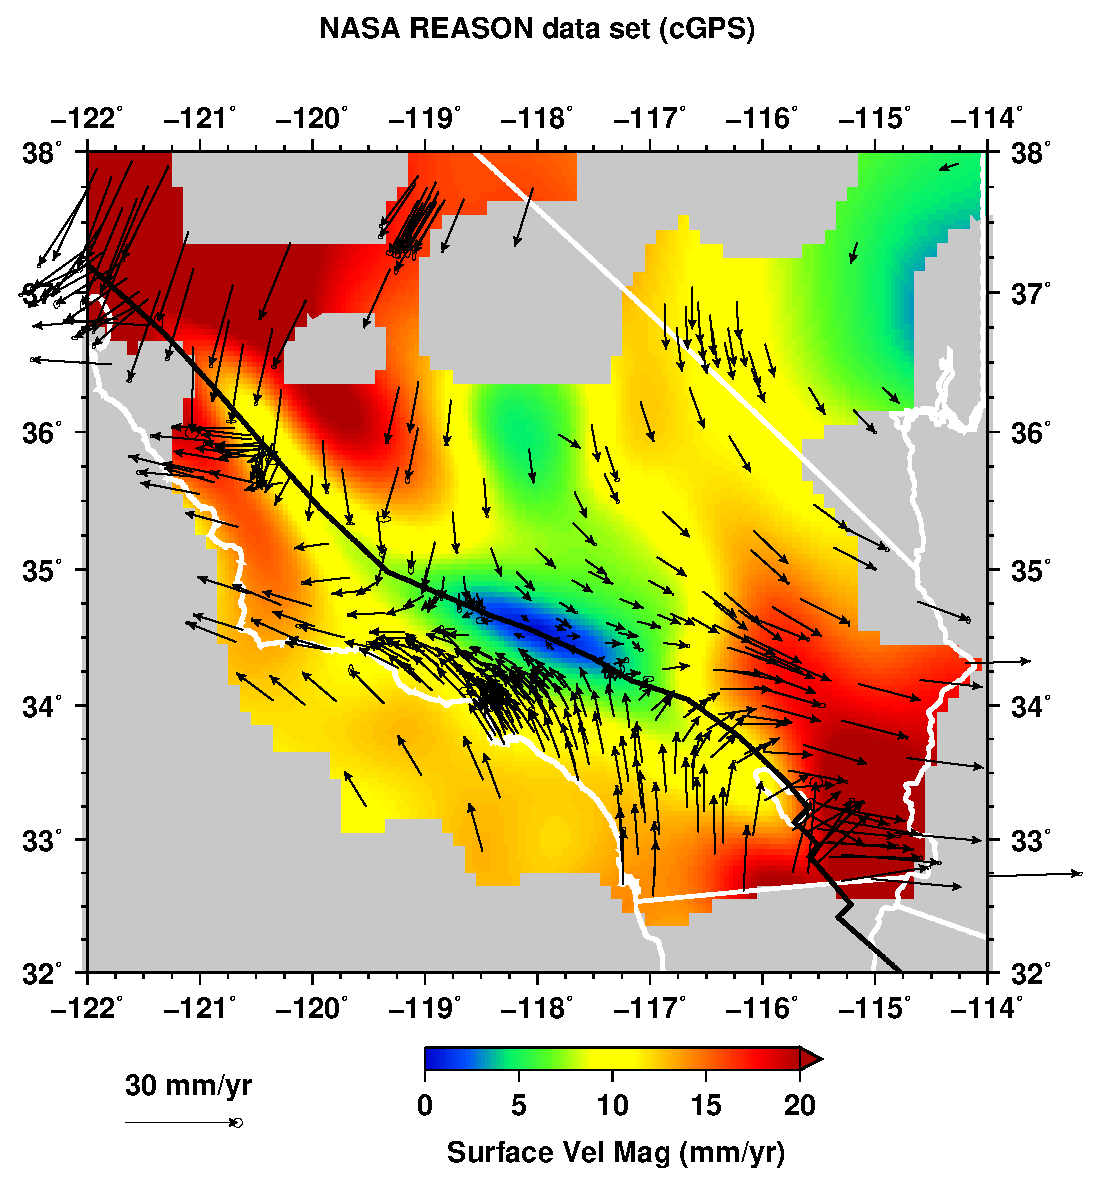
\includegraphics[width=16cm]{socal_d01_q03_q07_b1_2D_s1_u1_vfield.eps}
\caption[]
{{
Text.
\label{fig:2D_gmt1}
}}
\end{figure}

\begin{figure}
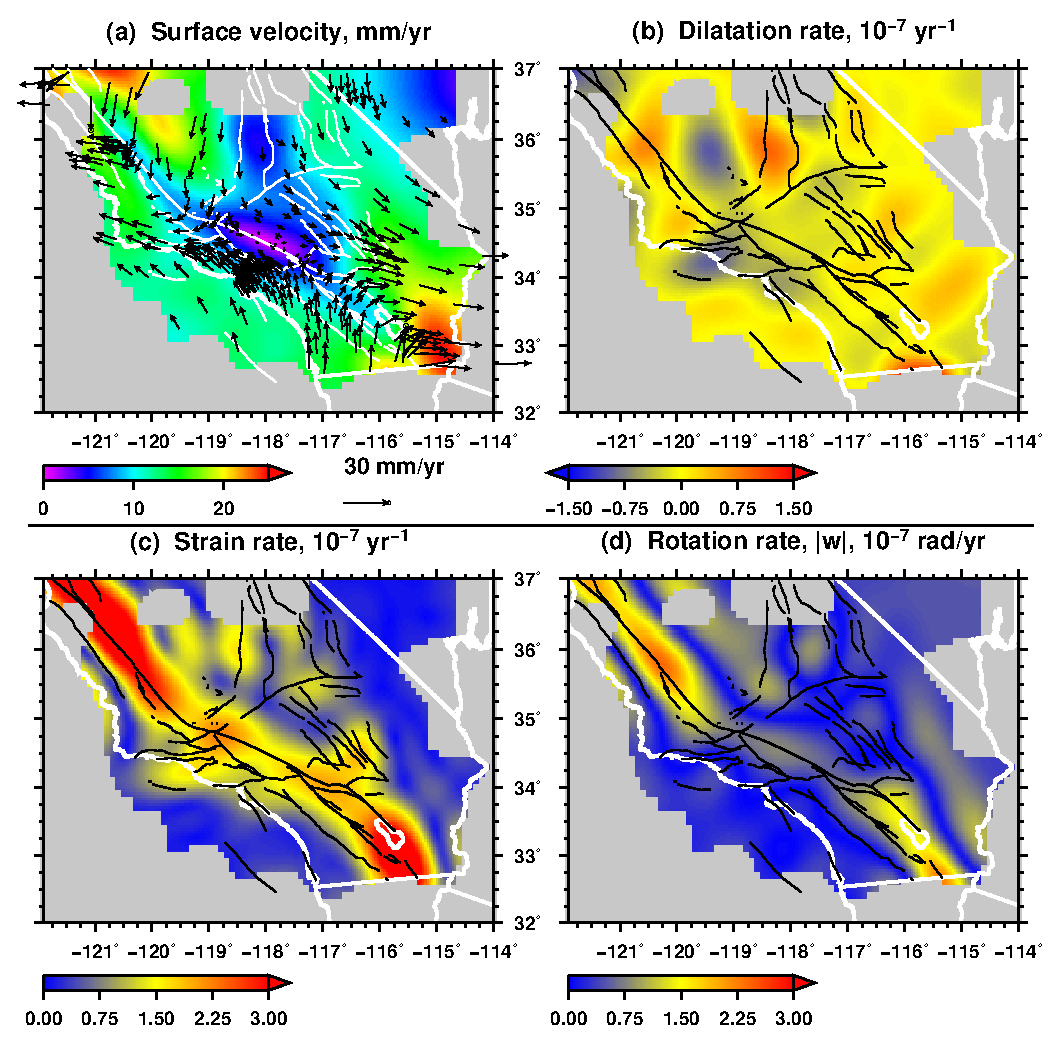
\includegraphics[width=16cm]{foursub_06_m1.eps}
\caption[]
{{
Text.
\label{fig:2D_gmt2}
}}
\end{figure}

%=====================================================
\end{document}
%=====================================================